\authorsection{General structure}{VI}

System must provide information having gathered data from users and other sources.
Application of complex algorithms is often necessary.
Amount of data and rate of its arrival are heavy.
Those aspects makes system to preprocess indices and aggregations that provide useful information.
Batch processing is a good solution for that, nevertheless it has drawback - execution time is long.
Incrementall processing resolves this issue.
In combination these two approaches allow to design a system, that answers user queries with low latency as well as accurate.

The purpose of the system is to answer queries having data.
Let's consider an artificial example.
Suppose we have a website where people pose programming questions, and other answer them.
In this case the simplest query to the system is to return list of answers for a particular question post.
Another query is to find all posts containing given keyword.

One query is easy to answer, another requires application of complex algorithms.
It is pretty easy to get list of answers to the question post having its id.
You simply create hash-table that maps questions' ids to lists of answers' ids.
Search by keyword, or even phrase search, is much more complex.
To make it possibe we have to build specific inverted index, and this requires much more time to execute and to programm.
Let's further assume, that our system has to provide keyword search, using precomputed inverted index. 

Amount of data gathered with the time, as well as intense of arrival, can be huge.
Let's consider again our example website.
Assume that on average every second 5 questions and 20 answers appear.
Every post is about 100 words, each of about 8 unicode symbols.
The rate of incoming data is then $25*100*8*2=39$ KB per second.
It is about 3.2 GB per day.
This leads our system to be able to process such amount of data efficiently, as well as to rapidly reflect the state of inverted index with newly arrived posts.

Amount of data and complexity of algorithms demand to make computations, useful for fast answering queries, in advance.
The system precomputes specific data structures, that provide data, prepared as much as possible to directly answer specific queries.
We call these data structures \textit{views}\mnote{view}.
They store indices and aggregations of original data.
In our example we consider inverted index as a view.
In a query time it provides efficient search of all posts with particular keyword.

The basic approach is to precompute views in a batch mode.
The \textit{batch layer} \mnote{batch layer} of the Lambda architecture is responsible for that.
It takes the whole dataset, available so far, and executes batch computations on it.
Views that are the result of batch processing we call \textit{batch views} \mnote{batch view}. 
This operation is efficient, because all data is at once in disposal.
We can execute any algorithm, and produce any kind of index or aggregation.
It is also easy to programm, because there are such greate approaches as MapReduce.
This paradighm is inherently distributed and scalable.
In example with website we would use MapReduce to create inverted index having all posts.
It requires only several lines of code in the simplest case.

After batch layer has precomputed views, it places them into the \textit{serving layer}\mnote{serving layer}.
The serving layer is responsible for storage of batch views.
It also provides interface to get particular data records from them. 

Batch layer starts then computations again, considering now data, that has come during the last batch processing.
This loop goes on infinitely.
Batch processing always starts again from scratch using all available data.
When the batch layer stores computed views into the serving layer, it discards old ones.

Figure~\ref{fig:lambda_architecture} depicts general view of the Lambda architecture. 

\begin{figure}
  \centering
  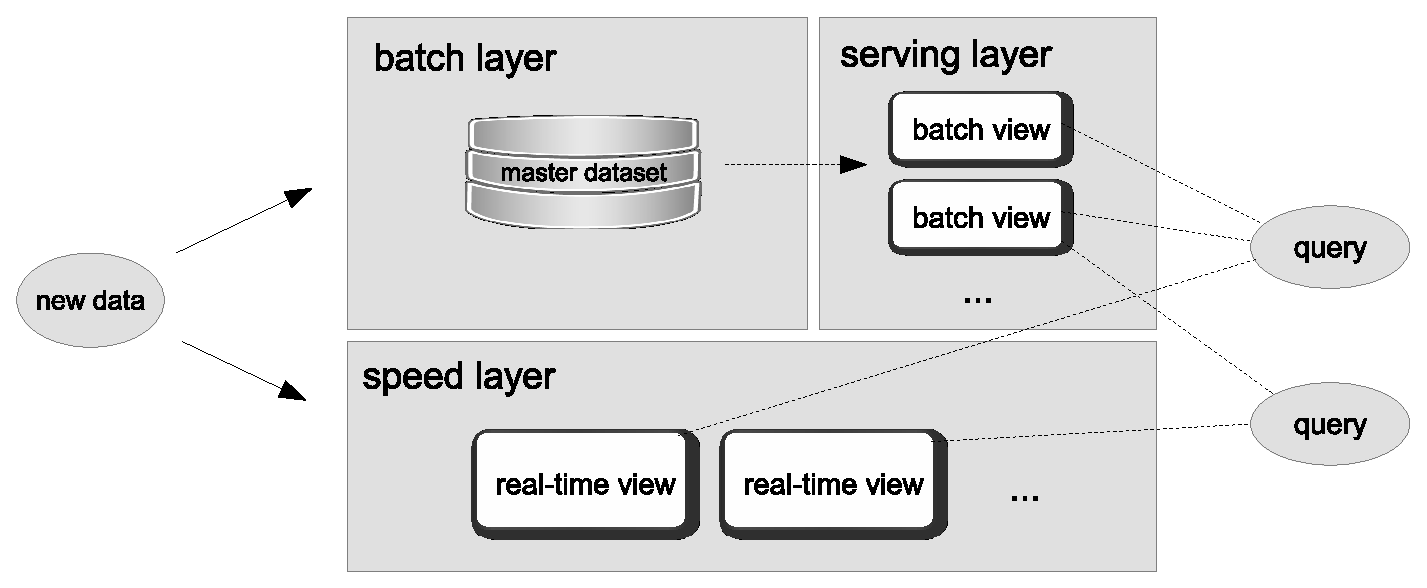
\includegraphics [width=1.0\textwidth]{images/LambdaArchitecture}
  \caption{General structure of the Lambda architecture. Batch and sevring layer are responsible for batch views, speed layer provides real-time views. To answer query system merges data from both types of views.}
  \label{fig:lambda_architecture}
\end{figure}

Batch computations, although easy and efficient, take long time to be done.
This cannot be underestimated, because on the BigData scale computations can last hours even if we setup cluster of thousends of machines.
In website example, assume our system has already been working for a year.
It has then about 800 millions of posts.
If we have a cluster of 100 machines, each has then to perform map-function 8 millions times.
If one execution of map-function takes 1 milisecond, it leads to 2.2 hours of total computations.
And we have not even counted reduce-phase.

As long as batch computations take much time, views are always outdated for several hours.
During this time new data arrives to the system, and it must be also counted in query answers.
This is not possible to solve using only batch processing.
Therefore, another approach is to apply.

To overcome delay of batch computations the Lambda architecture has additional component - the \textit{speed layer}\mnote{speed layer}.
It also computes views, but in incremental fashion.
We call them \textit{real-time views} \mnote{real-time view}.
As new data arrives, the speed layer updates incrementally real-time views.
Hence, they always has information from data, gathered during current batch processing.

Finally, to answer queries system uses both batch and real-time views.
Batch views contain result of the last batch processing.
Real-time views provide infromation from data, gathered after the beginning of the current batch processing.
Merging both types of views, system produces accurate and actual answers to the queries.